\documentclass[12pt]{beamer}

\usepackage[english]{babel}
\usepackage[utf8]{inputenc}

\usepackage{tikz}
\usetikzlibrary{shapes.symbols}

\bibliographystyle{amsalpha}

\usetheme{Copenhagen}
\setbeamertemplate{navigation symbols}{}
\setbeamertemplate{bibliography entry title}{}
\setbeamertemplate{bibliography entry location}{}
\setbeamertemplate{bibliography entry note}{}

\title{The FLP Theorem}
\author[Jacopo Notarstefano]{
  Jacopo Notarstefano\\
  \texttt{jacopo.notarstefano [at] gmail.com}
}
\date{November 26, 2014}

\begin{document}
  \begin{frame}[plain]
    \titlepage
  \end{frame}

  \begin{frame}{The Distributed Consensus Problem}
    Let's consider the problem of reaching agreement on a single value in a
    distributed, asynchronous system of processes.

    \vspace{0.25cm}

    For example, in a distributed database, all entities that have partecipated
    in the processing of a particular transaction need to agree wether to
    commit or rollback.

    \vspace{0.25cm}

    Whatever decision is made, all entities must make the same decision in
    order to preserve the consistency of the database.
  \end{frame}

  \begin{frame}{Faults}

    In this course we usually assumed that the partecipating processes and the
    network were completely reliable.

    \vspace{0.25cm}

    This is not the case with real systems, which are subject to a number of
    possible \textbf{faults}, such as process crashes, network partitioning,
    and lost, distorted, duplicated messages.

    \vspace{0.25cm}

    One can even consider \textbf{Byzantine} types of failures, in which faulty
    processes might go completely haywire, perhaps sending messages according
    to some malevolent plan \cite{LSP82}.
  \end{frame}

  \begin{frame}{The FLP Theorem}
    In 1985, Michael Fischer, Nancy Lynch, and Michael Paterson proved the
    surprising result that no completely asynchronous consensus protocol can
    tolerate even a single unannounced process death \cite{FLP85}.

    \vspace{0.25cm}

    Their proof did not consider Byzantine failures, and assumed that the
    message system is reliable — it delivers all messages correctly and exactly
    once.

    \vspace{0.25cm}

    Nevertheless, even with these assumptions, the stopping of a single process
    at an inopportune time can cause any distributed consensus protocol to fail
    to reach agreement.
  \end{frame}

  \begin{frame}{Consensus protocol}
    A \textbf{consensus protocol} is an asynchronous system of \(N\) processes
    (\(N\ge 2\)). Each process \(p\) has a one-bit \textbf{input register}
    \(x_p\), an \textbf{output register} \(y_p\) with values in \(\{\bot, 0,
    1\}\) and an unbounded amount of internal storage.

    \vspace{0.25cm}

    \textbf{Initial states} prescribe fixed starting values for all but the
    input register; in particular, the output register starts with value
    \(\bot\).

    \vspace{0.25cm}

    \(p\) acts deterministically according to a \textbf{transition} function.
  \end{frame}

  \begin{frame}{Decision states}
    The states in which the output register has value \(0\) or \(1\) are
    distinguished as being \textbf{decision states}. The transition function
    cannot change the value of the output register once the process has reached
    a decision state; that is, the output register is ``write-once''.

    \vspace{0.25cm}

    \begin{figure}
      \makebox[\textwidth][c]{
        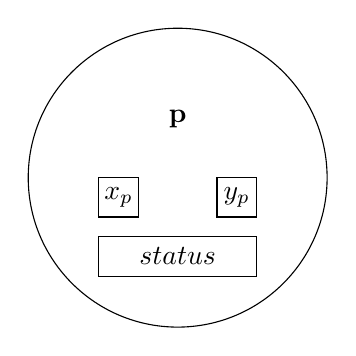
\begin{tikzpicture}
          \tikzstyle{process}=[circle, draw, inner sep=0pt, minimum size=108pt]

          \node (p) at (0, 0) [process] {};
          \node (plabel) at (0, 0.75) [] {\(\mathbf{p}\)};
          \node (xp) at (-0.75, -0.25) [] {\(x_p\)};
          \node (yp) at ( 0.75, -0.25) [] {\(y_p\)};
          \node (status) at (0, -1) [] {\(\text{status}\)};

          \draw (-1, -0.5) -- (-1, 0) -- (-0.5, 0) -- (-0.5, -0.5) -- cycle;
          \draw ( 1, -0.5) -- ( 1, 0) -- ( 0.5, 0) -- ( 0.5, -0.5) -- cycle;
          \draw (-1, -1.25) -- (-1, -0.75) -- (1, -0.75) -- (1, -1.25) -- cycle;
        \end{tikzpicture}
      }
    \end{figure}
  \end{frame}

  \begin{frame}{Message system}
    A \textbf{message} is a pair \((p,m)\), where \(p\) is the name of the
    destination process and \(m\) is a ``message value'' from a fixed universe
    \(M\).

    \vspace{0.25cm}

    The \textbf{message system} mantains a multiset, called the \textbf{message
    buffer}, of messages that have been sent but not yet delivered. It supports
    two abstract operations:
    \begin{description}
      \item[\texttt{ send(p,m)}:] Places \((p,m)\) in the message buffer.
      \item[\texttt{receive(p)}:] Deletes some message \((p,m)\) from the
        buffer and returns \(m\), in which case we say \((p,m)\) is
        \textbf{delivered}, or returns the special null marker \(\varnothing\)
        and leaves the buffer unchanged.
    \end{description}
  \end{frame}

  \begin{frame}{Nondeterministic messaging}
    The message system acts nondeterministically, subject only to the condition
    that if \texttt{receive(p)} is performed infinitely many times, then every
    message \((p,m)\) in the message buffer is eventually delivered.

    \vspace{0.25cm}

    \begin{figure}
      \makebox[\textwidth][c]{
        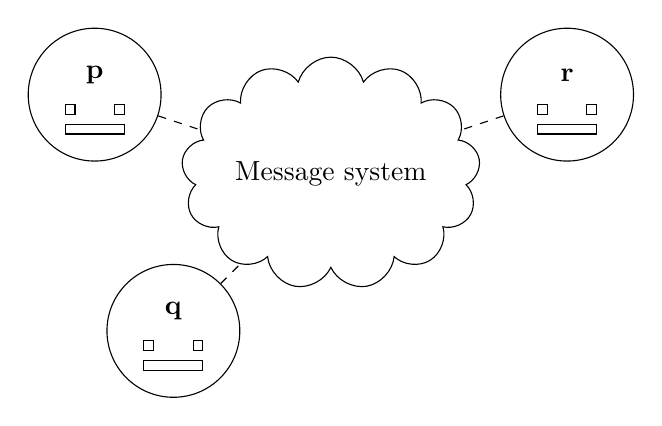
\begin{tikzpicture}
          \tikzstyle{process}=[draw, circle, inner sep=0pt, minimum size=48pt]
          \tikzstyle{system}=[draw, cloud, cloud puffs=13, inner sep=0pt, minimum width=108pt, minimum height=84pt]

          \node (system) at (0, 0) [system] {};
          \node (systemlabel) at (0, 0) [] {Message system};

          \node (p) at (-3,  1) [process] {};
          \node (plabel) at (-3, 1.25) [] {\(\mathbf{p}\)};
          \draw (-3.375, 0.875) -- (-3.375, 0.75) -- (-3.25, 0.75) -- (-3.25, 0.875) -- cycle;
          \draw (-2.625, 0.875) -- (-2.625, 0.75) -- (-2.75, 0.75) -- (-2.75, 0.875) -- cycle;
          \draw (-3.375, 0.625) -- (-3.375, 0.5) -- (-2.625, 0.5) -- (-2.625, 0.625) -- cycle;

          \node (q) at (-2, -2) [process] {};
          \node (qlabel) at (-2, -1.75) [] {\(\mathbf{q}\)};
          \draw (-2.375, -2.125) -- (-2.375, -2.25) -- (-2.25, -2.25) -- (-2.25, -2.125) -- cycle;
          \draw (-1.625, -2.125) -- (-1.625, -2.25) -- (-1.75, -2.25) -- (-1.75, -2.125) -- cycle;
          \draw (-2.375, -2.375) -- (-2.375, -2.5) -- (-1.625, -2.5) -- (-1.625, -2.375) -- cycle;

          \node (r) at ( 3,  1) [process] {};
          \node (rlabel) at (3, 1.25) [] {\(\mathbf{r}\)};
          \draw (3.375, 0.875) -- (3.375, 0.75) -- (3.25, 0.75) -- (3.25, 0.875) -- cycle;
          \draw (2.625, 0.875) -- (2.625, 0.75) -- (2.75, 0.75) -- (2.75, 0.875) -- cycle;
          \draw (3.375, 0.625) -- (3.375, 0.5) -- (2.625, 0.5) -- (2.625, 0.625) -- cycle;

          \draw (p) -- (system) [dashed] {};
          \draw (q) -- (system) [dashed] {};
          \draw (r) -- (system) [dashed] {};
        \end{tikzpicture}
      }
    \end{figure}
  \end{frame}

  \begin{frame}{Configurations and steps}
    A \textbf{configuration} of the system consists of the internal state of
    each process, together with the contents of the message buffer. An
    \textbf{initial configuration} is one in which each process starts at an
    initial state and the message buffer is empty.

    \vspace{0.5cm}

    A \textbf{step} takes one configuration to another and consists of a
    primitive step by a single process \(p\).
  \end{frame}

  \begin{frame}{Primitive steps and applicable events}
    Let \(C\) be a configuration. A step consists of two phases:
    \begin{enumerate}
      \item A \texttt{receive(p)} is performed on the message buffer in \(C\)
        to obtain a value \(m\in M\cup\{\varnothing\}\).
      \item Depending on \(p\)'s internal state in \(C\) and on \(m\), \(p\)
        enters a new internal state and sends a finite set of messages to other
        processes.
    \end{enumerate}

    \vspace{0.25cm}

    The step is completely determined by the pair \(e = (p,m)\), which we call
    an \textbf{event}.

    \vspace{0.25cm}

    An event \(e\) that \emph{could happen} at configuration \(C\) is called
    \textbf{applicable}, and the resulting configuration is denoted \(e(C)\).
  \end{frame}

  \begin{frame}{Schedules and runs}
    A \textbf{schedule} from \(C\) is a finite or infinite sequences \(\sigma\)
    of applicable events, in turn, starting from \(C\). The associated sequence
    of steps is called a \textbf{run}.

    \vspace{0.25cm}

    If \(\sigma\) is finite, we let \(\sigma(C)\) denote the resulting
    configuration, which is said to be \textbf{reachable} from \(C\).

    \vspace{0.25cm}

    A configuration reachable from some initial configuration is said to be
    \textbf{accessible}.
  \end{frame}

  \begin{frame}{Partial correctness}
    A configuration \(C\) has \textbf{decision value} \(v\) if some process
    \(p\) is in a decision state with \(y_p = v\).

    \vspace{0.25cm}

    \begin{definition}[Partial correctness]
      A consensus protocol is \textbf{partially correct} if:
      \begin{enumerate}
        \item No accessible configuration has more than one decision value.
        \item For each \(v\in \{0,1\}\), some accessible configuration has decision value \(v\).
      \end{enumerate}
    \end{definition}
  \end{frame}

  \begin{frame}{Total correctness in spite of one fault}
    A process \(p\) is \textbf{nonfaulty} in run if it takes infinitely many
    steps, otherwise it is \textbf{faulty}.

    \vspace{0.25cm}

    A run is \textbf{admissible} if at most one process is faulty and all
    messages sent to nonfaulty processes are eventually received.

    \vspace{0.25cm}

    A run is \textbf{deciding} if some process reaches a decision state.

    \vspace{0.25cm}

    \begin{definition}[Total correctness in spite of one fault]
      A consensus protocol \(P\) is \textbf{totaly correct in spite of one
      fault} if it is partially correct and every admissibile run is deciding.
    \end{definition}
  \end{frame}

  \begin{frame}{Main result}
    \begin{theorem}[Fischer, Lynch, Paterson 1985]
      No consensus protocol is totally correct in spite of one fault.
    \end{theorem}

    \vspace{0.25cm}

    A configuration is \textbf{bivalent} if the set of decision values of
    configurations reachable from it has \(2\) elements. It is instead
    \textbf{\(0\)-valent} or \textbf{\(1\)-valent} according to the
    corresponding value.

    \vspace{0.25cm}

    \begin{proof}[Proof (sketch)]
      Given an initial bivalent configuration, we construct an admissible run
      that at each stage results in another bivalent configuration.
    \end{proof}
  \end{frame}

  \begin{frame}{Lemma 1}
    \begin{lemma}
      Suppose that from some configuration \(C\), the schedules \(\sigma_1\),
      \(\sigma_2\) lead to configurations \(C_1\), \(C_2\) respectively. If the
      sets of processes taking steps in \(\sigma_1\) and \(\sigma_2\),
      respectively, are disjoint, then \(\sigma_2\) can be applied to \(C_1\)
      and \(\sigma_1\) can be applied to \(C_2\), and both lead to the same
      configuration \(C_3\).
    \end{lemma}

    \vspace{0.25cm}

    In other words: \textbf{schedules about disjoint processes commute with
    each other}.
  \end{frame}

  \begin{frame}{Proof of Lemma 1}
    \begin{figure}
      \makebox[\textwidth][c]{
        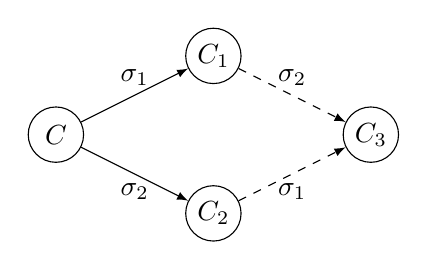
\begin{tikzpicture}
          \tikzstyle{configuration}=[draw,circle,inner sep=0pt,minimum size=20pt]

          \node (C) at (0,0) [configuration] {\(C\)};
          \node (C1) at (2,1) [configuration] {\(C_1\)};
          \node (C2) at (2,-1) [configuration] {\(C_2\)};
          \node (C3) at (4,0) [configuration] {\(C_3\)};

          \draw[-latex] (C) to node[above] {\(\sigma_1\)} (C1);
          \draw[-latex] (C) to node[below] {\(\sigma_2\)} (C2);
          \draw[-latex, dashed] (C1) to node[above] {\(\sigma_2\)} (C3);
          \draw[-latex, dashed] (C2) to node[below] {\(\sigma_1\)} (C3);
        \end{tikzpicture}
      }
    \end{figure}

    Because the sets of processes are disjoint, an event in \(\sigma_1\)
    applicable to \(C\) is applicable to \(C_2\) as well.

    \vspace{0.25cm}

    Because of determinism, after all events are processed they must end up in
    the same state. \qed

  \end{frame}

  \begin{frame}{Lemma 2}
    \begin{lemma}
      \(P\) has a bivalent initial configuration.
    \end{lemma}

    \vspace{0.25cm}

    Assume by contradiction that there isn't. Then, by partial correctness,
    \(P\) must have both \(0\)-valent and \(1\)-valent initial configurations.

    \vspace{0.25cm}

    Let's call two initial configurations \textbf{adjacent} if they differ only
    in the initial value \(x_p\) of a single process \(p\). Any two initial
    configurations are joined by a chain of inital configurations, each
    adjacent to the next.
  \end{frame}

  \begin{frame}{Proof of Lemma 2}
    Hence, there must exist a \(0\)-valent initial configuration \(C_0\)
    adjacent to a \(1\)-valent configuration \(C_1\). Let \(p\) be the process
    in whose initial value they differ.

    \vspace{0.25cm}

    Consider some admissibile deciding run from \(C_0\) in which process \(p\)
    takes no steps, and let \(\sigma\) be the associated schedule. Then
    \(\sigma\) can be applied to \(C_1\) as well, and the corresponding
    configurations will be identical except for \(p\)'s internal state.

    \vspace{0.25cm}

    Both runs reach the same decision value; if it is \(1\) then \(C_0\) was
    bivalent, if it is \(0\) then \(C_1\) was bivalent. \qed
  \end{frame}

  \begin{frame}{Lemma 3}
    \begin{lemma}
      Let \(C\) be a bivalent configuration of \(P\), and let \(e = (p,m)\) be
      an event that is applicable to \(C\). Let \(\mathcal{C}\) be the set of
      configurations reachable from \(C\) without applying \(e\), and let
      \(\mathcal{D} = e(\mathcal{C}) = \{ e(E)\;\vert\;E \in \mathcal{C} \text{
      and } e \text{ is applicable to \(E\)} \}\). Then, \(\mathcal{D}\)
      contains a bivalent configuration.
    \end{lemma}

    \vspace{0.25cm}

    In other words: given a bivalent configuration and an event \(e\)
    applicable to it, \textbf{we construct another bivalent configuration
    having \(e\) as the last applied event}.
  \end{frame}

  \begin{frame}{Proof of Lemma 3}
    Assume by contradiction that \(\mathcal{D}\) contains no bivalent
    configuration. We first show that \(\mathcal{D}\) contains both
    \(0\)-valent and \(1\)-valent configurations.

    \vspace{0.25cm}

    Let \(E_i\) be an \(i\)-valent configuration from \(C\). If \(E_i\in
    \mathcal{C}\), let \(F_i = e(E_i) \in \mathcal{D}\). Otherwise \(e\) was
    applied in reaching \(E_i\), and so there exists \(F_i \in \mathcal{D}\)
    from which \(E_i\) is reachable.

    \vspace{0.25cm}

    In either case, \(F_i\) is \(i\)-valent since it is in \(\mathcal{D}\),
    which contains no bivalent configuration by hypothesis.
  \end{frame}

  \begin{frame}{Proof of Lemma 3}
    We call two configurations \textbf{neighbors} if one results from the other
    in a single step. Then there exists neighbors \(C_0, C_1\in\mathcal{C}\)
    such that \(D_i = e(C_i)\) is \(i\)-valent for \(i = 0,1\). WLOG, we can
    assume \(C_1 = e'(C_0)\) where \(e' = (p, m)\).

    \vspace{0.25cm}

    If \(p \neq p'\), then \(D_1 = e'(D_0)\) by Lemma 1. This is impossible,
    since a successor of a \(0\)-valent configuration is \(0\)-valent.

    \vspace{0.25cm}

    If instead \(p = p'\), then consider any finite deciding run from \(C_0\)
    in which \(p\) takes no steps. Let \(\sigma\) be the corresponding
    schedule, and let \(A = \sigma(C_0)\).
  \end{frame}

  \begin{frame}{Proof of Lemma 3}
    By Lemma 1, \(\sigma\) is applicable to \(D_i\) and leads to an
    \(i\)-valent configuration \(E_i = \sigma(D_i)\) for \(i = 0,1\).

    \vspace{0.25cm}

    Also by Lemma 1, \(e(A) = E_0\) and \(e(e'(A)) = E_1\). Hence, \(A\) is
    bivalent, a contradiction.

    \vspace{0.25cm}

    \begin{figure}
      \makebox[\textwidth][c]{
        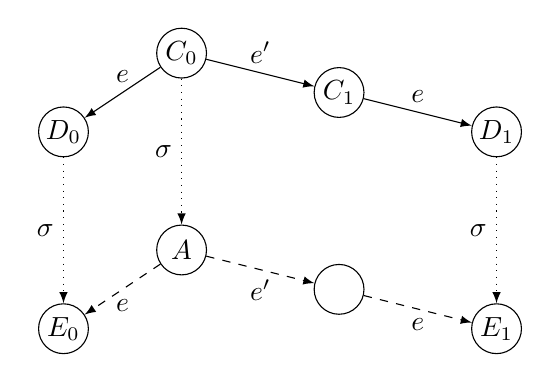
\begin{tikzpicture}
          \tikzstyle{configuration}=[draw, circle, inner sep=0pt, minimum size=18pt]

          \node (A) at (0, 0) [configuration] {\(A\)};
          \node (C0) at (0, 2.5) [configuration] {\(C_0\)};
          \node (D0) at (-1.5, 1.5) [configuration] {\(D_0\)};
          \node (E0) at (-1.5, -1) [configuration] {\(E_0\)};
          \node (C1) at (2, 2) [configuration] {\(C_1\)};
          \node (F1) at (2, -0.5) [configuration] {};
          \node (D1) at (4, 1.5) [configuration] {\(D_1\)};
          \node (E1) at (4, -1) [configuration] {\(E_1\)};

          \draw[-latex] (C0) to node[above] {\(e'\)} (C1);
          \draw[-latex] (C0) to node[above] {\(e\)} (D0);
          \draw[-latex] (C1) to node[above] {\(e\)} (D1);

          \draw[-latex, dotted] (D0) to node[left] {\(\sigma\)} (E0);
          \draw[-latex, dotted] (C0) to node[left] {\(\sigma\)} (A);
          \draw[-latex, dotted] (D1) to node[left] {\(\sigma\)} (E1);

          \draw[-latex, dashed] (A) to node[below] {\(e\)} (E0);
          \draw[-latex, dashed] (A) to node[below] {\(e'\)} (F1);
          \draw[-latex, dashed] (F1) to node[below] {\(e\)} (E1);
        \end{tikzpicture}
      }
    \end{figure}
  \end{frame}

  \begin{frame}{Proof of main result}
    TODO
  \end{frame}

  \begin{frame}{Conclusions}
    TODO
  \end{frame}

  \begin{frame}{Bibliography}
    \bibliography{seminar.bib}
  \end{frame}
\end{document}
